% !TEX root = week_1.tex
% !TeX encoding = UTF-8
% !TeX spellcheck = en_US
\documentclass[a4paper]{scrartcl}
\usepackage[T1]{fontenc}
%\usepackage[utf8]{inputenc}
\usepackage[english]{babel}
\usepackage[bottom=2.5cm,top=2.0cm,left=2.0cm,right=2.0cm]{geometry}
\usepackage{amssymb,amsmath,amsfonts}
\usepackage{lmodern}
\usepackage{csquotes}
\usepackage{url}
\usepackage{doi}
\usepackage{hyperref}
\usepackage{enumitem}
\usepackage{graphicx}
\usepackage[dvipsnames]{xcolor}
\definecolor{mygreen}{rgb}{0,0.4,0}
\definecolor{mygray}{rgb}{0.5,0.5,0.5}
\usepackage[numbered,framed]{matlab-prettifier}
\usepackage[backend=biber,style=authoryear]{biblatex}
\addbibresource{literature/_biblio.bib}
\usepackage[stable]{footmisc}
\usepackage{booktabs,longtable}
\usepackage{nameref}
\usepackage{float}
\usepackage{tikz}
\usetikzlibrary{positioning}
\usetikzlibrary{decorations.text}
\renewcommand{\contentsname}{Overview}

\usepackage[
	%nosolutionfiles
	]{answers}

\Newassociation{solution}{Solution}{week_1_solution}
\newif\ifDisplaySolutions\DisplaySolutionstrue

\begin{document}
\title{Quantitative Macroeconomics\\~\\Winter 2023/24\\~\\Week 1}
\author{Willi Mutschler\\willi@mutschler.eu}
\date{Version: 1.0.0\\Latest version available on: \href{https://github.com/wmutschl/Quantitative-Macroeconomics/releases/latest/download/week_1.pdf}{GitHub}}
\maketitle\thispagestyle{empty}

\newpage
\Opensolutionfile{week_1_solution}[week_1_solution]
\tableofcontents\thispagestyle{empty}\newpage

\setcounter{page}{1}
\section[What is Quantitative Macroeconomics]{What is Quantitative Macroeconomics\label{ex:QuantitativeMacroeconomics}}
Broadly define the scope and research topics of \enquote{Quantitative Macroeconomics},
  sometimes referred to as \enquote{Macroeconometrics}. What are
\begin{itemize}
  \item \textbf{S}tructural \textbf{V}ector \textbf{A}uto\textbf{R}egressive models?
  \item \textbf{D}ynamic \textbf{S}tochastic \textbf{G}eneral \textbf{E}quilibrium models?
  \item the challenges and approaches in estimating SVAR and DSGE models?  
\end{itemize}

\paragraph{Readings}
\begin{itemize}
  \item \textcite{Cantore.Gabriel.Levine.EtAl_2013_ScienceArtDSGE}
  \item \textcite{Christiano.Eichenbaum.Trabandt_2018_DSGEModels}
	\item \textcite{Fernandez-Villaverde.Rubio-Ramirez_2010_StructuralVectorAutoregressions}
	\item \textcite{Guerron-Quintana.Nason_2013_BayesianEstimationDSGE}
	\item \textcite[Ch. 1]{Herbst.Schorfheide_2016_BayesianEstimationDSGE}
	\item \textcite{Kilian_2013_StructuralVectorAutoregressions}
	\item \textcite[Ch. 1, Ch. 6]{Kilian.Lutkepohl_2017_StructuralVectorAutoregressive}
	\item \textcite{Schorfheide_2010_BayesianMethodsMacroeconometrics}
\end{itemize}

\begin{solution}\textbf{Solution to \nameref{ex:QuantitativeMacroeconomics}}
\ifDisplaySolutions
Quantitative macroeconomics combines (i) modern theoretical macroeconomics
  (the study of aggregated variables such as economic growth, unemployment and inflation
  by means of structural macroeconomic models)
  with (ii) state-of-the-art econometric methods (the application of formal statistical methods in empirical economics).
To this end, we will focus on the two workhorse model frameworks, namely SVAR and DSGE,
  and develop the numerical procedures and algorithms required to estimate such models.
Very important: this course is \textbf{NOT ABOUT HOW TO BUILT} structural models,
  but it is \textbf{ABOUT HOW TO ESTIMATE} such models using real data.

This enables us to look at abstract macroeconomic concepts, for example:
\begin{itemize}
  \item Is uncertainty a source of business cycles or an endogenous response to them, and does the type of uncertainty matter?
  What are the effects on the real price of oil and on macroeconomic aggregates of
    oil supply shocks, shocks to the global demand for all industrial commodities,
    or demand shocks that are specific to the crude oil market?
  That is, we want to understand the propagation of shocks by means of an \textbf{impulse response analysis}.
  In other words, we want to \textbf{quantify} the dynamic effect of identified and economic meaningful shocks over time.
  For example:\\\includegraphics*[width=\textwidth]{plots/NarrativeSignRestrictionsIRFs.png}
  \item How important are monetary policy shocks as opposed to other shocks for movements in aggregate output?
  That is, we want to identify sources of fluctuations by means of a \textbf{variance decomposition}.
  In other words, we want to \textbf{quantify} how important a shock is on explaining the variation in the endogenous variables \textbf{on average}.
  For example:
  \begin{center}  
  \begin{tabular}{@{}llllll@{}}
  \toprule
                & \multicolumn{5}{c}{Shocks}                                      \\ \midrule
                & Monetary & Technology & Preference & Price markup & Wage markup \\
  Output growth & 4.8\%    & 22.3\%     & 57.1\%     & 8.0\%        & 7.1\%       \\
  Inflation     & 27.1\%   & 6.1\%      & 36.3\%     & 13.7\%       & 14.7\%      \\
  Nominal rate  & 5.0\%    & 0.4\%      & 72.3\%     & 9.8\%        & 11.8\%      \\
  Hours         & 0.4\%    & 0.8\%      & 70.0\%     & 17.6\%       & 9.6\%       \\
  Wage          & 0.1\%    & 0.1\%      & 73.6\%     & 12.0\%       & 12.8\%      \\ \bottomrule
  \end{tabular}
  \end{center}
  \item Has monetary policy changed in the early 1980s? Has it caused the 1982 recession?
  That is, we want to study how much a given structural shock explains the historically observed fluctuations in aggregate variables
    at every given point in time by means of a \textbf{historical decomposition}.    
  In other words, we want to \textbf{quantify} how important a shock was in driving the behavior of the endogenous variables in a \textbf{specific time period in the past}.
  For example:\\\includegraphics*[width=\textwidth]{plots/Historical-Decomposition-of-Aggregate-Hours-Worked.jpeg}
  \item To what extent would the financial crises have deepened if monetary policy had not responded to the output contraction at all?
  That is, we want to study \textbf{counterfactual policies}.
  \item How will inflation, growth and unemployment evolve over the next eight quarters?
  That is, we want to predict the values of variables in the future by means of a \textbf{forecast}.  
\end{itemize}

\paragraph*{Traditional Cowles Commission approach}
The prevailing econometric framework was initiated and developed in the 1950s to 1970s by the Cowles Commission by inventing
  many things such as indirect least squares, instrumental variable methods, the full and the limited information maximum likelihood methods.
Broadly speaking they developed the theory and toolkits (based on linear regressions) for estimating large-scale system of equations
  that have a certain structure that enables one to estimate these simultaneous equations one-by-one.
The IS-LM or AS-AD models are examples of such systems,
  where we have some underlying ad-hoc assumptions (e.g. consumption is always equal to a fraction of current output)
  that give us a reduced-form from which we can compute things like fiscal policy multipliers.
This reduced-form also enables us to estimate these parameters.
Of course, these models are useful for gaining intuition,
  but are quite limited for actual \textbf{quantitative} policy advise
  and analysis of how the whole economy responds to particular shocks or policies.
Nevertheless, these models were (and still are\footnote{
  More elaborated versions of such models are still in use at central banks and policy institutions under the label of semi-structural models.})
  empirically somewhat successful when measured in terms of forecast quality.
However, as the ultimate goal in macroeconomics is to gain policy insight and to actually understand the transmission channels,
  this approach came under heavy attack in the mid 1970s by (i) \textcite{Lucas_1976_EconometricPolicyEvaluation} and (ii) \textcite{Sims_1980_MacroeconomicsReality}:
\begin{itemize}
  \item Sims critique: many restrictions that are used to identify behavioral equations in these models are inconsistent with dynamic macroeconomic theories
  $\rightarrow$ (structural) vector autoregressions ((S)VAR)
  \item Lucas critique: models are unreliable for policy analysis
  because they are unable to predict effects of policy regime changes on the expectation formation of economic agents in a coherent manner
  $\rightarrow$ development of micro-founded structural models is necessary
\end{itemize}

\paragraph*{SVAR approach}
Pioneered by Christopher \textcite{Sims_1980_MacroeconomicsReality}.
The basic idea is to model all endogenous variables JOINTLY rather than one equation at a time.
This breaks with the traditional so-called Cowles Commission approach that relies on ad-hoc assumptions to do equation-by-equation estimation,
  which in essence generates implausible exogeneity assumptions (think about estimating the IS-LM model).
The underlying statistical framework is the vector autoregressive model,
  i.e. we do multivariate linear regressions of a vector of observables on its own lags and (possibly) other variables such as a constant, trends or exogenous variables.
Importantly, we have cross-equation constraints that are jointly modeled and estimated.
This is the VAR framework.

Now adding the \textbf{S} to \textbf{VAR} means to add structure on the cross-equation restrictions,
  in order to differentiate between correlation and causation.
The basic idea is to decompose the forecast errors (i.e. the residuals) into so-called structural shocks
  that are mutually uncorrelated and have an economic interpretation (supply shocks, demand shocks, risk shocks, monetary policy shocks, rare disaster shocks, etc.).
More precisely, instead of given every parameter in the VAR model a behavioral interpretation,
  we make explicit identifying assumptions to isolate estimates of policy and/or private agent's behavior
  and its effects on the economy while keeping the model free of many additional restrictive assumptions.  
In principle, this enables us to analyze the causal effects of these structural shocks on the model variables by all kinds of objectives.
But of course, it all depends on the validity of the identifying assumptions.
Typically, these stem from institutional knowledge, economic theory or other extraneous constraints on the model responses.
Most of the recent literature is primarily concerned with finding new and more compelling identifying assumptions (or methods),
in order to consolidate or challenge known results.
The upside of the SVAR approach is that ideally, with very few assumptions about the structure of the economy, 
  we get meaningful and, above all, data-based results.

\paragraph*{DSGE approach}
DSGE models use modern macroeconomic theory to explain and predict co-movements of aggregate time series.
DSGE models start from what we call the micro-foundations of macroeconomics
  (i.e. to be consistent with the underlying behavior of economic agents),
  with a heart based on the rational expectation forward-looking economic behavior of agents.
The dynamic equilibrium is the result from the combination of economic decisions taken by all economic agents.
For example the following agents or sectors are commonly included:
\begin{itemize}
  \item Households: benefit from private consumption, leisure and possibly other things like money holdings or state services;
    subject to a budget constraint in which they finance their expenditures 
    via (utility-reducing) work, renting capital and buying (government) bonds
    $\hookrightarrow$ maximization of utility
  \item Firms produce a variety of products with the help of rented equipment (capital) and labor.
  They (possibly) have market power over their product and are responsible for
    the design, manufacture and price of their products.
    $\hookrightarrow$ cost minimization or profit maximization
  \item Monetary policy follows a feedback rule, so-called Taylor rule, for instance: 
    nominal interest rate reacts to deviations of the current (or lagged) inflation rate
    from its target and of current output from potential output
  \item Fiscal policy (the government) collects taxes from households and companies 
    in order to finance government expenditures (possibly utility-enhancing) 
    and government investment (possibly productivity-enhancing).
    In addition, the government can issue debt securities and might face a probability of sovereign default.
  \item There is no limitation, i.e. you can also add other sectors (financial, trade, R\&D, etc).
\end{itemize}
 We then mathematically solve these problems under uncertainty,
   because we add stochastic processes to the system of equations. 
\begin{itemize}
  \item General Equilibrium (GE): equations must always hold.
  \\
  Short-run: decisions, quantities and prices adjust such that equations are full-filled.
  \\
  Long-run: steady-state, i.e. a condition or situation where variables do not change their value 
  (e.g. balanced-growth path where the rate of growth is constant). 
  \item Stochastic (S): disturbances (or shocks) make the system deviate from its steady-state, 
  we get business cycles or, more general, a data-generating process
  \item Dynamic (D): Agents are forward-looking and solve intertemporal optimization problems. 
  When a disturbance hits the economy, macroeconomic variables do not return to equilibrium instantaneously, 
    but change very slowly over time, producing complex reactions. 
  Furthermore, some decisions like investment or saving only make sense in a dynamic context.
  We can analyze and quantify the effects after
		(i) a temporary shock: how does the economy return to its steady-state, or 
		(ii) a permanent shock: how does the economy move to a new steady-state.
\end{itemize}
DSGE models are intensively used in policy making e.g. by central banks they play a central role in providing an analytical foundation for the decision making.
They have become the standard modelling framework in modern macroeconomic research.
They often serve as a macroeconomic laboratory that allows to analyze how economic agents respond to changes in their environment
  as all variables are determined simultaneously and endogenously given a sound micro-founded theoretical setting.
Real business cycle (RBC) models, New Keynesian models, and asset pricing models
  all belong to this very general modelling class.

Estimating such models is a very challenging task as one has to first find a reduced-form suitable for estimation.
The upside, however, is that ideally, with suitable solution and estimation techniques,
  we have a clear theoretical foundation for our empirical results that enable clear understanding of transmissions channels and policy advise.

\paragraph*{Challenges in Quantitative Macroeconomics}
\begin{itemize}
  \item Macroeconomic time series are indicative of nonlinearities, non-Gaussianity and time-varying volatility.  
  \item Model specification: How to select the \enquote{right} model, how to cope with misspecification?
  \item SVAR
  \begin{itemize}
    \item many free parameters to estimate, need plausible identifying restrictions
    \item sensitive to the identification restrictions used
    \item risk of specification search: researchers look for reasonable answers or puzzles under the cloak of formal statistical inference
  \end{itemize}  
  \item DSGE
  \begin{itemize}
    \item trade-off between theoretical coherence and empirical fit
    \item heavily aggregated and stylized, require a lot of modelling assumptions
    \item solving DSGE models requires knowledge in computational eocnomics
  \end{itemize} 
  \item computational implementation is in both cases often cumbersome and challenging  
\end{itemize}
Despite the challenges and current developments,
  SVAR and DSGE models continue to be the fundamental tools in current macroeconomic analysis.
Be warned: there is quite the investment one needs to undergo to study quantitative macroeconomics
  and there is a huge component of self-teaching involved,
  because most of us lack the required background in econometrics, mathematics, numerics and statistics.
In fact, most macroeconomists doing research in this area are more or less self-taught (I can attest to this for myself),
  or come from a related field.
\fi
\newpage
\end{solution}\newpage
\section[Programming Languages]{Programming Languages\label{ex:ProgrammingLanguages}}
\begin{enumerate}
	\item Name some popular programming languages in macroeconomics.
	Which are general purpose, which are domain specific?
	\item What are the differences between compiled and interpreted languages?
	\item What is important when choosing a programming language for scientific computing in macroeconomics?
	Which programming language{(s)} would you choose?
\end{enumerate}

\paragraph{Readings}
\begin{itemize}
\item \textcite{Aguirre.Danielsson_2020_WhichProgrammingLanguage}
\item \textcite{Aruoba.Fernandez-Villaverde_2015_ComparisonProgrammingLanguages} (note the Update available at \url{https://www.sas.upenn.edu/~jesusfv/Update_March_23_2018.pdf})
\end{itemize}

\begin{solution}\textbf{Solution to \nameref{ex:ProgrammingLanguages}}
\ifDisplaySolutions%
\begin{enumerate}

\item
General purpose: C/C++, Python, Excel.
Domain-specific: MATLAB, Julia, R, Fortran, Mathematica, EViews.

\item
Every program is a set of instructions, say to add two numbers.
Compilers and interpreters take human-readable code and convert it to computer-readable machine code.
In a compiled language, the target machine directly translates the program.
In an interpreted language, the source code is not directly translated by the target machine.
Instead, a different program, aka the interpreter, reads and executes the code.
Some modern languages like Python can have both compiled and interpreted implementations,
  but for simplicity's sake it is useful to keep in mind the distinction.

Compiled languages like Fortran, C or C++ are usually fastest, more efficient and more powerful,
  but they are harder to learn and harder to code in.
They also require a build step, i.e.\ they need to be compiled.
Interpreted languages like Python, Mathematica, MATLAB, R or Julia are slower,
  but easier to learn and faster to code in.
Interpreters run through a program line by line and execute each command.
Interpreted languages tend to be very similar in the syntax,
  but differ in best practices and concepts.

Interpreted languages were once significantly slower than compiled languages.
But, with the development of just-in-time (JiT) compilation, that gap is shrinking.
MATLAB and Julia (and to some extent also Python and R) are very prominent examples that make use of JiT compilation,
  that is they combine both worlds.

While interpreted languages like Python or R are slower, they benefit from large libraries (e.g., NumPy, Pandas)
  that are implemented in highly optimized compiled languages like C/C++ or Fortran, mitigating the performance gap for many tasks.
You can also make use of e.g. Fortran or C++ code in MATLAB, R, Python or Julia;
  that is, write very CPU-intensive tasks in a compiled language
  and use them in an interpreted language.


\item
Learning a programming language is a huge investment;
  however, once one has knowledge of one, learning another one tends to be easier
  as they are based on similar principles.
Try to stick with popular choices as the choice of learning resources and communities
  that help you learn this language are wider spread,
  i.e.\ googling for help is much easier for Python than for Fortran.
Often the project you are working on dictates which programming language you should use.
The general purpose languages can be used in many non-scientific applications,
  so your investment might payoff in very different fields in the end.

In scientific computing, particularly in Macroeconomics,
  we are often faced with CPU intensive problems
  and need to prototype models and methods quickly.
An interpreted language like MATLAB or Julia that does just-in-time compilation
  is therefore best suited for such tasks.
Moreover, having some basic knowledge in C++ is advisable
  to write computational intensive tasks in a compiled language
  and reuse this inside interpreted languages.
However, the main determining factor is by looking at legacy code of the last 20--30 years of research done
  in quantitative and computational Macroeconomics,
  we see that most was and still is conducted in MATLAB,
  whereas highly intensive tasks were programmed in Fortran.
So keep in mind, that you need to understand this legacy codebase.
In the last couple of years, Julia has gained traction in Macroeconomics,
  but new developments like Machine Learning require you to invest in Python.
For writing scientific reports and papers you should get familiar with Latex and Markdown.

Another issue to consider is the license, cost and support of the language maintainers.
Most programming languages are free and open-source,
  others like MATLAB are proprietary and are quite expensive
  (free and open-source clones like Octave tend to be very slow unfortunately).
Regardless of the license, having a good governance structure,
  i.e.\ a board, cooperation or company driving the development of the language,
  is very important for the sustainability of the language
  and for your investment in a computer language.

Lastly, and very importantly, have a look at the tools available for the languages.
Which Integrated Development Environment (IDE) do you like best?
Which code editor do you prefer?
How good are the debugging capabilities of your chosen environment.
Things like syntax highlighting, smart indentation, code linting, comparison tools,
  handling of workspace, etc.\ are very important.
Some languages like MATLAB bring their own IDE in one big package and it works very well,
Others like Julia, Python or C++ can be neatly integrated in a variety of environments;
  in fact Visual Studio Code has become the leading editor and environment for many languages,
  but of course there are many other great choices depending on your needs and preferences.
  (e.g.\ there is PyCharm for Python or RStudio for R).

So which computer languages should you devote your time into,
  if you are interested in computational or quantitative macroeconomics?
\\
\textbf{Here is my opinionated advice:}
\begin{itemize}
\item Default languages (excellent knowledge): Julia and MATLAB
\item Data analysis and Machine Learning (advanced knowledge): R and Python
\item Heavy tasks (basic knowledge): C++ and Fortran
\item Scientific writing (advanced knowledge): Latex and Markdown
\end{itemize}

\end{enumerate}
\fi
\newpage
\end{solution}\newpage
\section[Quick Tour: MATLAB]{Quick Tour: MATLAB\label{ex:QuickTourMATLAB}}
Install the most recent version of MATLAB with the following Toolboxes:
	Econometrics Toolbox,
	Global Optimization Toolbox,
	Optimization Toolbox,
	Parallel Computing Toolbox,
	Statistics and Machine Learning Toolbox,
	Symbolic Math Toolbox. Open a new script and do the following:
\footnote{If you don't have any previous programming experience,
  I would highly recommend to go through
  \textcite[Appendix A]{Brandimarte_2006_NumericalMethodsFinance},
  \textcite[Appendix B]{Miranda.Fackler_2002_AppliedComputationalEconomics},
  and \textcite{Pfeifer_2017_MATLABHandout}.}

\begin{enumerate}
	\item Define the column vectors
	\begin{align*}
		x &=\left( -1,0,1,4,9,2,1,4.5,1.1,-0.9\right)' && y =\left( 1,1,2,2,3,3,4,4,5,\text{nan}\right)'
	\end{align*}
	\item Check if both vectors have the same length using either \texttt{length()} or \texttt{size()}. 
	\item Perform the following logical operations:
	\begin{align*}
		x &<y &&
		x <0 &&
		x+3 \geq 0 &&
		y <0
	\end{align*}
	\item Check if all elements in x satisfy both $x+3\geq 0$ and $y>0$.
	\item Check if all elements in x satisfy either $x+3\geq 0$ or $y>0$.
	\item Check if at least one element of $y$ is greater than $0$.
	\item Compute $x+y$, $xy$, $xy'$, $x'y$, $y/x$, and $x/y$.
	\item Compute the element-wise product and division of $x$ and $y$.
	\item Compute $\ln (x)$ and $e^x$.
	\item Use \texttt{any} to check if the vector $x$ contains elements	satisfying $\sqrt{x}\geq 2$.
	\item Compute
	$a =\sum_{i=1}^{10}x_{i}$ and $b =\sum_{i=1}^{10}y_{i}^{2}$.
	Omit the nan in $y$ when computing the sum.
	\item Compute $\sum_{i=1}^{10}x_{i}y_{i}^{2}$.
	Omit the nan in $y$ when computing the sum.
	\item Count the number of elements of $x>0$.
	\item Predict what the following commands will return:
	\begin{verbatim}x.^y  	x.^(1/y)  	log(exp(y))  	y*[-1,1]  	x+[-1,0,1]   sum(y*[-1,1],1,'omitnan') \end{verbatim} 	
	\item Define the matrix
 	$X=\begin{pmatrix}
 	1 & 4 & 7 \\ 
 	2 & 5 & 8 \\ 
 	3 & 6 & 9
 	\end{pmatrix}$.
	Print the transpose, dimensions and determinant of $X$.
	\item Compute the trace of $X$ (i.e. the sum of its diagonal elements).
	\item Change the diagonal elements of $X$ to [7,8,9].
	\item Compute the eigenvalues of (the new) $X$.
	Display a message if $X$ is positive or negative definite.
	\item Invert $X$ and compute the eigenvalues of $X^{-1}$.
	\item Define the column vector $a=(1,3,2)'$ and compute \texttt{a'*X}, \texttt{a'.*X}, and \texttt{X*a}.
	\item Compute the quadratic form $a^{\prime }Xa$.
	\item Define the matrices
 		$I=\left[ 
 		\begin{array}{lll}
 		1 & 0 & 0 \\ 
 		0 & 1 & 0 \\ 
 		0 & 0 & 1
 		\end{array}
 		\right]$,
 		$Y=\left[ 
 		\begin{array}{lll}
 		1 & 4 & 7 \\ 
 		2 & 5 & 8 \\ 
 		3 & 6 & 9
 		\end{array}
 		\begin{array}{lll}
 		1 & 0 & 0 \\ 
 		0 & 1 & 0 \\ 
 		0 & 0 & 1
 		\end{array}
 		\right]$ and $Z=\left[ 
 		\begin{array}{lll}
 		1 & 4 & 7 \\ 
 		2 & 5 & 8 \\ 
 		3 & 6 & 9 \\
 		1 & 0 & 0 \\ 
 		0 & 1 & 0 \\ 
 		0 & 0 & 1
 		\end{array}
 		\right]$.
	\item Generate the vectors
	\begin{align*}
 		x_{1} &=\left( 1,2,3,\ldots ,9\right) ,&&
 		x_{2} =\left( 0,1,0,1,0,1,0,1\right) ,&&
 		x_{3} =\left( 1,1,1,1,1,1,1,1\right) \\
 		x_{4} &=\left( -1,1,-1,1,-1,1\right) ,&&
 		x_{5} =\left( 1980,1985,1990,\ldots ,2010\right) ,&&
 		x_{6} =\left( 0,0.01,0.02,\ldots ,0.99,1\right)
	\end{align*}
	using sequence operator \texttt{:} or \texttt{repmat}.
	\item Generate a grid of $n=500$ equidistant points on the interval $[-\pi,\pi ]$ using \texttt{linspace}.
	\item Compare \texttt{1:10+1}, \texttt{(1:10)+1} and \texttt{1:(10+1)}.	
	\item Define the following column vectors
 		\begin{align*}
 		x&=
 		\begin{pmatrix}
 		1 &
 		1.1 & 
 		9 & 
 		8 & 
 		1 & 
 		4 & 
 		4 & 
 		1
 		\end{pmatrix} ,\quad y=
 		\begin{pmatrix}
 		1 & 
 		2 & 
 		3 & 
 		4 & 
 		4 & 
 		3 & 
 		2 & 
 		\text{NaN}
 		\end{pmatrix}'
		 \\ z&=
 		\begin{pmatrix}
 		true & 
 		true & 
 		false & 
 		false & 
 		true & 
 		false & 
 		false & 
 		false
 		\end{pmatrix}'
 		\end{align*}
 	\item Predict what the following commands will return (and then check if you are right):\\
 	\texttt{x(2:5)}, \texttt{x(4:end-2)}, \texttt{x([1 5 8])}, \texttt{x(repmat(1:3,1,4))},\\
	 \texttt{y(z)}, \texttt{y(\textasciitilde z)}, \texttt{y(x>2)}, \texttt{y(x==1)},\\
	 \texttt{x(\textasciitilde isnan(y))}, \texttt{y(\textasciitilde isnan(y))}
	\item Indexing is not only used to read certain elements of a vector but also to change them.
	Execute \texttt{x2 = x} to make a copy of \texttt{x}. Change all elements of \texttt{x2} that have the value $4$ to the value $-4$. Print \texttt{x2}.
	\item Change all elements of \texttt{x2} that have the value 1 to a missing value (\texttt{nan}). Print \texttt{x2}.
	\item Execute \texttt{x2(z) = []}. Print \texttt{x2}.
	\item Define the matrix $M = \begin{pmatrix}
		1&     5&     9&    12&     8&     4\\
		2&     6&    10&    11&     7&     3\\
		3&     7&    11&    10&     6&     2\\
		4&     8&    12&     9&     5&     1 \end{pmatrix}$
		using the $:$ operator and the \texttt{reshape} command.
	\item Predict what the following commands will return (and then check if you are right):\\
	\texttt{M(1,3)},
	\texttt{M(:,5)},
	\texttt{M(2,:)},
	\texttt{M(2:3,3:4)},
	\texttt{M(2:4,4)},
	\texttt{M(M>5)},
	\texttt{M(:,M(1,:)<=5)},
	\texttt{M(M(:,2)>6,:)},
	\texttt{M(M(:,2)>6,4:6)}
	\item Print all rows of $M$ where column 5 is at least three times larger than column 6.
	\item Count the number of elements of $M$ that are larger than 7.
	\item Count the number of elements of $M$ in row 2 that are smaller than their neighbors in row 1.
	\item Count the number of elements of $M$ that are larger than their left neighbor.
\end{enumerate}


\paragraph{Readings}
\begin{itemize}
	\item \textcite[Appendix A]{Brandimarte_2006_NumericalMethodsFinance}.
	\item \textcite[Appendix B]{Miranda.Fackler_2002_AppliedComputationalEconomics}.
	\item \textcite{Pfeifer_2017_MATLABHandout}
\end{itemize}

\begin{solution}\textbf{Solution to \nameref{ex:QuickTourMATLAB}}
\ifDisplaySolutions
\lstinputlisting[style=Matlab-editor,basicstyle=\mlttfamily]{progs/matlab/quickTourMatlab.m}
\fi
\newpage
\end{solution}\newpage
\section[Quick Tour: git with GitKraken]{Quick Tour: git with GitKraken (OPTIONAL)\label{ex:QuickTourGitWithGitKraken}}

\begin{enumerate}

\item
What is \emph{git}? What is \emph{GitKraken}? What is \emph{GitHub}?

\item
How does a typical workflow in Quantitative Macroeconomics look like?
How can a version control system like git support this workflow?

\item
If you haven't already, sign up for a free account on GitHub: \url{https://github.com/signup}

\item
If you haven't already, sign up for the GitHub Student Developer Pack \url{https://education.github.com/pack}.
If you add your university email address, the decision process is very fast (usually within a day).

\item
Install GitKraken for your operating system \url{https://www.gitkraken.com/download} and connect it with GitHub.
Go to preferences \(\rightarrow \) Integrations \(\rightarrow \) GitHub and click \emph{Generate SSH key and add to GitHub}.
Checkout the other preferences.
For instance, if you are on Windows make sure that under \emph{Editor} the \emph{End of Line Character} is set to \emph{LF}.\footnote{%
  If you are on Windows and working with people who are not (or vice-versa),
    you'll probably run into line-ending issues at some point.
  This is because Windows uses both a carriage-return character and a linefeed character for newlines in its files,
    whereas macOS and Linux systems use only the linefeed character.
  This is a subtle but incredibly annoying fact of cross-platform work;
    many editors on Windows silently replace existing LF-style line endings with CRLF,
    or insert both line-ending characters when the user hits the enter key.
  Therefore, it is advised to tell git to convert CRLF to LF on commit but not the other way around.
}

\item
Create a local repository on your computer called \emph{Quant-Macro} by selecting \texttt{Start a local repo} in GitKraken.

\item
With your favorite text editor open the \texttt{README.md} file inside the folder and add the following:
\begin{lstlisting}[basicstyle=\scriptsize\mlttfamily]
# Repository for Quantitative Macroeconomics
In this repository I will practice estimating SVAR and DSGE models.
The folder contains examples and codes developed in the lecture.
But I still don't understand git and find this really cumbersome!
Dropbox, iCloud, Nextcloud, and OneDrive is so much better!
\end{lstlisting}
Save the file and have a look into GitKraken what happened in your repository.

\item
Explain the \emph{git model} of staging, committing and pushing.

\item
Stage and commit all the changes you made so far to the repository.

\item
What is a \emph{good commit}?

\item
\emph{Soft Reset} your current status (so-called HEAD) to the initial commit.
Re-commit everything except the last line in the README.md file without actually changing the file in your text editor.
Put the remaining changes (i.e.\ the last line into the stash, which is a place for work-in-progress).

\item
Push your local repository to GitHub and visit https://github.com/[USERNAME]/Quant-Macro to see what happened.

\item
What are \emph{git branches}?
Create a branch called \emph{latex-exam-template} and checkout the branch.

\item
While on your \emph{latex-exam-template} branch, use your favorite text editor
  to create the three files \texttt{templateExamSolution.tex}, \texttt{templateExamBiblio.bib}, and \texttt{templateMatlabExample.m} given in the Appendix.
Typically, when copy and pasting from a pdf you will run into characters (like minus signs and empty space) not correctly pasted into your text editor,
  so you will need to check everything manually.
Once you are happy, commit only three files using the message \enquote{Created latex template for exam solutions}.

\item
Compile the Latex files using your favorite Latex GUI or via the command line:
\begin{lstlisting}[language=tex,frame=single,basicstyle=\scriptsize\mlttfamily]
pdflatex templateExamSolution
biber templateExamSolution
pdflatex templateExamSolution
pdflatex templateExamSolution
\end{lstlisting}
Open the pdf to make sure the file compiled correctly.

\item
Like in the previous exercise we often have some auxiliary files created by a program which we do not care about.
We can tell \emph{git} to ignore individual files or patterns of files.
In GitKraken, simply right-click on the file you want to ignore and select how you want to ignore it.
Do so for the just created auxiliary Latex files, but also for the generated pdf (as it is binary).
Have a look into the newly created \texttt{.gitignore} file and commit it.\footnote{%
  GitHub also has a collection of useful gitignore files for various programming languages at \url{https://github.com/github/gitignore}.
}

\item
Create a Pull Request to GitHub of your develop branch to your main branch. Go to GitHub and accept this.
See what happens in the repository.

\item
Switch back to your main branch and pull the merged changes.
Then click Pop to add the changes you had in your stash back on top of the current branch.
Either decide to discard the last line in the README.md file or commit it and schedule a meeting with me to discuss your issues.

\item
Once you got accepted to the GitHub Student Developer Pack, activate GitKraken to get the free PRO license.

\end{enumerate}


\paragraph{Readings}
\begin{itemize}
\item \url{https://www.gitkraken.com/learn/git}: highly recommended (particularly the videos)
\item \textcite{Chacon_2014_ProGit}: extensive book on git
\end{itemize}

\paragraph{Useful urls}
\begin{itemize}	
\item \url{https://www.sas.upenn.edu/~jesusfv/Chapter_HPC_5_Git.pdf}
\item \url{https://github.com/jaredgars/LEAP}
\item \url{https://luispfonseca.com/files/slides_git.pdf}
\item \url{https://www.frankpinter.com/notes/git-for-economists-presentation.pdf}
\item \url{https://github.com/fditraglia/git-for-economists}
\item \url{https://matteosostero.com/files/slides_git.pdf}
\end{itemize}

\begin{solution}\textbf{Solution to \nameref{ex:QuickTourGitWithGitKraken}}
\ifDisplaySolutions%
\begin{enumerate}

\item
\emph{git} is a version control system, i.e.\ a way to track changes to code, text, documents, data etc.
It let's you go back and forth between many different versions of the same file, and see a list of the differences.
Collaboration becomes (technically) very easy and straightforward as people can work on different files or different versions of the same file simultaneously
  and afterwards merge their changes.

\emph{git} is the most popular version control system invented in 2005 to track the development of the worldwide largest open-source project: the Linux Kernel.
It is a \textbf{command line tool}, and at some point you should learn the commands on the Command Line Interface (CLI).
However, there are many graphical user interface (GUI) programs that make getting started with Git much easier
  and integrate seamlessly with online collaboration platforms such as GitHub or GitLab.
Therefore, in this exercise I will focus on such a tool called GitKraken,
  which I use daily and highly recommend.\footnote{%
  Other GUI programs work very similarly,
    see \url{https://en.wikipedia.org/wiki/Comparison_of_Git_GUIs} for a comparison of features.
  I also recommend the built-in git functionality of Visual Studio Code.
}
GitKraken offers a free trial of their paid license,
  but also offers a free version for use on publicly-hosted repositories (which is fine for our purposes as we will mostly do stuff locally anyway).
Additionally, GitKraken also offers the Pro license FREE to students and teachers through the GitHub Student Developer Pack (\url{https://education.github.com/pack}).

While git and GitKraken are tools that you install on your computer,
  GitHub is an online platform that provides a nice visual interface to help you manage your version-controlled projects remotely.
It is the largest git repository hosting service and has become by far the largest open-source collaboration site.
Another important online platform is Gitlab as you can also host that on your computer or server.
For individuals gitea offers yet another way to host a stripped down version of GitHub or Gitlab.	
I personally have accounts on GitHub (\url{https://github.com/wmutschl}) and Gitlab (\url{https://gitlab.com/wmutschl}),
  but also use self-hosted versions of Gitlab (\url{https://git.dynare.org/wmutschl}) and gitea (\url{https://git.mutschler.eu}) to mirror my projects.

\item
A typical workflow looks like this:
\begin{itemize}
\item retrieve data and prepare it for estimation purposes
\item select a model framework, decide on certain hyper-parameters and modeling choices and then run an estimation
\item prepare tables, graphs and reports
\end{itemize}
All of these tasks heavily rely on coding, i.e.\ putting text into some files that are then evaluated by software that actually performs the tasks.
Moreover, we will see that simulating macroeconomic models requires a lot of trial and error and accordingly those files constantly change and need to be adapted.
\emph{git} enables you to track these changes as it gives you an organized revision history.
So you can experiment with your codes, make changes to a project and always keep the ability to go back and fourth between changes.
So stop naming files like \emph{2024{-}04{-}24-master-thesis-v2-final-now-really-final.tex}
  and let \emph{git} do its magic for you by simply tracking the file \emph{thesis.tex} with all of its revision history.

\item
Follow the instructions provided in the links or get in touch if you are struggling with the installation.

\item
Follow the instructions provided in the links or get in touch if you are struggling with the installation.

\item
Follow the instructions provided in the links or get in touch if you are struggling with the installation.

\item
In GitKraken: Open a new Tab, click \emph{Start a local repo}, then on the \emph{Init} register select \emph{Local Only} and fill out the details.
Note that GitKraken automatically creates a first commit with a \texttt{README.md} file.
Inside every repository there is a hidden folder \texttt{.git}.
It contains everything done by \emph{git}, so all the changes you will ever do.
Never delete this folder!
Also putting a repository on a cloud storage folder might damage this folder,
  so best practice is to use a local folder on the disk.
We will cover how to push the repository to a so-called remote which works basically like syncing,
  but much more robust and git-ier.

\item
Now the benefits of using a GUI like GitKraken become evident,
  as our changes are displayed in the \emph{Unstaged Files} area
  and by clicking on the file we get a really pretty side-by-side comparison of all the changes.
We can now decide which lines we want to \texttt{stage} and \texttt{commit}.

\item
The git model looks like the following diagram:\\
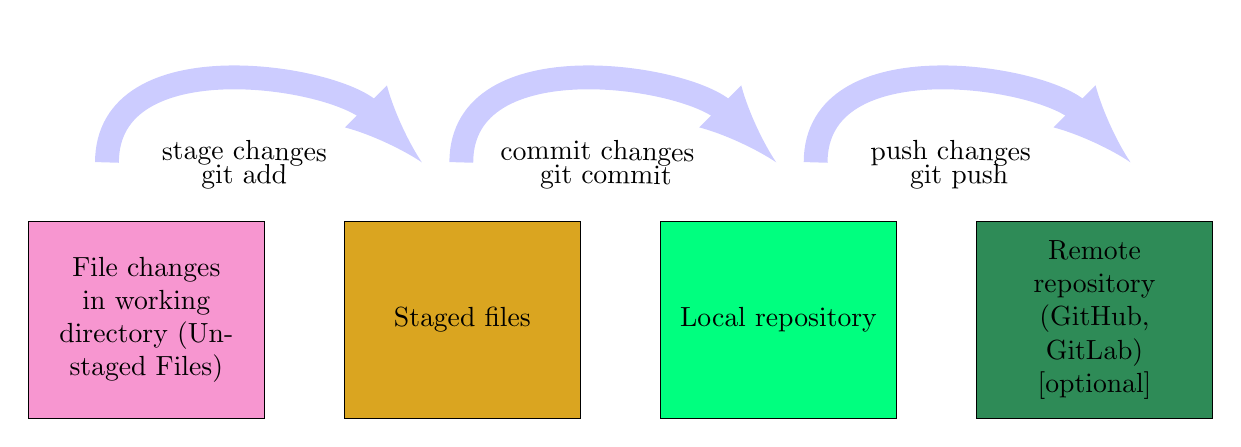
\begin{tikzpicture}[mypostaction/.style 2 args={decoration={text align={left indent=#1}, text along path, text={#2}},decorate}]
\node[draw,
      fill=Rhodamine!50,
      minimum width=3cm,
      minimum height=2.5cm,
      text width=2.5cm,
      text centered
     ]
	 (unstaged) at (0,0) {File changes in working directory (Unstaged Files)};
\node [draw,
       fill=Goldenrod,
	   minimum width=3cm,
	   minimum height=2.5cm,
	   text width=2.5cm,
	   text centered,
	   right=1cm of unstaged
	  ]
	  (staged) {Staged files};	 
\node [draw,
	   fill=SpringGreen, 
	   minimum width=3cm, 
	   minimum height=2.5cm,
	   text width=2.5cm,
	   text centered,
	   right=1cm of staged
	  ]
	  (local) {Local repository};	 
\node [draw,
       fill=SeaGreen, 
	   minimum width=3cm, 
	   minimum height=2.5cm,
	   text width=2.5cm,
	   text centered,
	   right=1cm of local
	  ]
	  (remote) {Remote repository (GitHub, GitLab) [optional]};
	 
% Arrows with text label
\coordinate (unstageRoot) at (-0.5,2); \coordinate (stageRoot) at (3.5,2);
	\draw[-latex, blue!20!white, line width=2ex]  (unstageRoot) to[in=135,out=90] (stageRoot);
	\path [postaction={mypostaction={0.7cm}{stage changes}},postaction={mypostaction={1.2cm}{git add},/pgf/decoration/raise=-3mm}](unstageRoot) to [in=180,out=3] (stageRoot);
\coordinate (stageRoot) at (4,2); \coordinate (localRoot) at (8,2);
	\draw[-latex, blue!20!white, line width=2ex]  (stageRoot) to[in=135,out=90] (localRoot);
	\path [postaction={mypostaction={0.5cm}{commit changes}},postaction={mypostaction={1cm}{git commit},/pgf/decoration/raise=-3mm}](stageRoot) to [in=180,out=3] (localRoot);
\coordinate (localRoot) at (8.5,2); \coordinate (remoteRoot) at (12.5,2);
	\draw[-latex, blue!20!white, line width=2ex]  (localRoot) to[in=135,out=90] (remoteRoot);
	\path [postaction={mypostaction={0.7cm}{push changes}},postaction={mypostaction={1.2cm}{git push},/pgf/decoration/raise=-3mm}](localRoot) to [in=180,out=3] (remoteRoot);

\end{tikzpicture}

You do your work in your \textbf{working directory}.
On the \textbf{stage} you collect all the changes that you want to save.
This is very powerful because sometimes it is just individual lines of code or text that you want to keep track of and not the whole file.
Once you've tracked all the changes that you want to combine, it is time to collect these changes into a \textbf{commit}.
A commit is a permanent snapshot of the files that git tracks stored in the {.git} directory.
It is associated with a unique identifier (hash).
In other words, a commit is like a snapshot in time; you can always revert back to this and see what changes were made compared to any other commit.
On your local repository (i.e.\ on your local machine) you now have a nice versioned history.
However, if you want to collaborate with others or sync your repository to a specialized cloud provider you need to push these changes to a so-called remote repository,
  typically on GitHub, GitLab, but any folder that you can access via remotely might serve as a remote repository.

\item
Click on the file and select \texttt{Stage File} or add each line by clicking on the plus or minus signs left to each line.
Once you are happy with the file, click on the X to close the file-comparison window.
We now don't see any unstaged files and can proceed to write a commit message and then click on the big green button.

\item
A \emph{good commit} typically does one discrete task or change only.
For example, you added a variable to the regression specification in the code, in the output and in the report.
Or you changed the name of a variable and treat it properly across multiple scripts.
This enables you to make meaningful commit messages like \emph{Add wage rigidities to the model} or \emph{Fix bug in the simulation routine}
  and you thus end up with a well organized repository.
This workflow needs some practice and everyone is slightly different with regards to this.
Nevertheless, try to combine changes to certain meaningful smaller tasks and provide good commit messages.
In my experience, having ten tiny commits is always preferable to one large commit.
Your future self and collaborators will thank you!

The question to what you should include in your commits, is also a matter of choice and preference.
Definitely your script files of codes, latex and text files.
Data is also sometimes given as csv files which are basically just text files.
Binary files (like Excel sheets, Word documents, Power Point slides) are a bit tricky to handle,
  as you can't see the differences between versions in git.
It depends on the specific needs whether one should commit these files as well (e.g.\ for Excel files with data this obviously makes sense),but I usually don't do this.
Note that GitHub doesn't allow files larger than 100 MB or projects with total size larger than 1 {GB}.
There is also a way to deal with large binary files called \texttt{Git Large File Storage (LFS)}.

\item
Right click on the initial commit and select \emph{Reset main to this commit {-} Soft}.
Click on the file in the staged files section and remove the last line from the stage.
Re-commit your stage by providing a meaningful commit message and hitting the green button.
Click on Stash to put the remaining changes into the stash.

\item
Simply click on Push and add the remote.
On the left Panel click on REMOTE to see the current remote (usually named origin).
Note that you can add several remotes (say from different people) and compare the commits.
Remotes are also a nice backup of your codes.

\item
Branches are arguably the most powerful part of \emph{git}.
By default you have a \textbf{main} branch,
  but what if you want to do some experiments, re-write an estimation function from scratch, work on a new feature, etc?
You could copy the whole folder and start working there or you use git and create a branch and make the changes there.
You can switch between branches, make commits to any branch, move them around, etc.
If your experiment doesn't work out, simply delete the branch.
If your experiments work out, commit them and merge them into the main branch.
Sometimes there will be conflicts which one needs to sort out,
  but using GUI tools like GitKraken makes this very easy
  as you have a pretty side-by-side comparison of changes.
Branches are arguably the most powerful part of \emph{git} especially for our purposes
  as research is a highly nonlinear process, and this way of doing version control is much more similar to how we actually work
  than the very linear way that other cloud storage providers do version control.
Branches are also extremely powerful for collaboration
  as different people can work on the same thing at the same time.

Select a so-called parent commit, where you want to create a new branch.
Note that this doesn't have to be the latest commit.
Click on the button \emph{Branch} and name it according to the exercise.
On the left panel, click on LOCAL to see an overview of all your branches.

\item
Create, copy and paste the three files into your repository.
Check for pasting errors and then \emph{Stage all changes} and commit them.

\item
Run the commands and solve any errors you might get from latex.

\item
Follow the instructions in the exercise.
Note that there is a difference between \enquote{Ignore} and \enquote{Ignore and Stop Tracking}.
\enquote{Ignore} simply adds the file{(type)} to the \texttt{.gitignore} file so that new files with that name/type/whatever are not tracked.
To \enquote{Ignore and Stop Tracking} means to remove the file{(s)} from git version control:
  they will no longer be in the repo (as of the commit that performs the \enquote{stop tracking}).
Basically, use \enquote{Ignore and Stop Tracking} if the file{(s)} you are ignoring never should have been in the repo in the first place.

\item
Make sure you are on the correct branch \emph{latex-exam-template} and push this branch to GitHub.
Either right click on the commit or go to the left panel, click on PULL REQUESTS and on the green plus sign that appears.
Select the \emph{latex-exam-template} as the FROM REPO branch and \emph{main} as the TO REPO branch.
Enter a Title and Description and click on the green button.
Have a look in GitHub ar the pull request.
As there are no conflicts merge it and go back to GitKraken to see what happens in your repository.
You might need to \enquote{fetch origin} by right clicking on the origin remote.

\item
Double click on your local main branch and then click on pull,
  which fast forwards your repo to the merged changes.
Then click on Pop to get the WIP codes which were stored on main.
Right click on the README.md file in the \emph{Unstaged Files} area and select \emph{Discard changes}.

\end{enumerate}
\fi
\newpage
\end{solution}\newpage
\printbibliography
\newpage
\appendix
\section{Exam template files for \LaTeX}
\lstinputlisting[language=tex,frame=single,title=\lstname,breaklines=true,breakatwhitespace=false,basicstyle=\scriptsize\mlttfamily]{progs/latex/template_exam_solution.tex}
\lstinputlisting[language=tex,frame=single,title=\lstname,breaklines=false,breakatwhitespace=false,basicstyle=\scriptsize\mlttfamily]{progs/latex/template_exam_biblio.bib}
\lstinputlisting[style=Matlab-editor,basicstyle=\footnotesize\mlttfamily,title=\lstname]{progs/matlab/template_matlab_example.m}

\Closesolutionfile{week_1_solution}
\ifDisplaySolutions
\newpage
\section{Solutions}
\input{week_1_solution}
\fi
\end{document}